\documentclass[a4paper]{article}

%--------------------------------------------------------------------------

\usepackage[a4paper, total={6in, 9in}]{geometry}
\usepackage{amsmath}
\usepackage{booktabs}
\usepackage{caption}
\usepackage{enumitem}
\usepackage{graphicx}
\usepackage{float}
\usepackage{inconsolata}
\usepackage{listings}
\usepackage{pstricks-add}
\usepackage{siunitx}
\usepackage[most]{tcolorbox}
\usepackage{tikz}
\usepackage{epstopdf} %converting to PDF
\usepackage{hyperref}
\usepackage{makecell}
\usepackage{siunitx}
\usepackage{wrapfig}

\usetikzlibrary{shapes.geometric}

%------------------------------------------------------------
\graphicspath{{./fig/}}

%------------------------------------------------------------
\setlength{\parindent}{0in}

\lstdefinestyle{Python}{
	language        = Python,
	basicstyle      = \ttfamily,
	keywordstyle    = \color{blue},
	keywordstyle    = [2] \color{teal}, % just to check that it works
	stringstyle     = \color{green},
	commentstyle    = \color{red}\ttfamily
}

%------------------------------------------------------------
\newtcblisting[auto counter]{sexylisting}[2][]{sharp corners, 
    fonttitle=\bfseries, colframe=gray, listing only, 
    listing options={basicstyle=\ttfamily,language=Python}, 
    title=Listing \thetcbcounter: #2, #1}

%--------------------------------------------------------------------------

\begin{document}
\title{Udacity: Follow Me Report}
\author{Shane Reynolds}
\maketitle
\tableofcontents

\newpage

\section{Introduction}
Computer vision is a subset of robotic perception - it has been defined as the development of autonomous systems which can perform tasks achieved by human visual systems (Huang, 1996). This means the acquisition of digital image data from an optical camera, and some type of interpretation of the acquired image. A simple example of a task that is routinely performed by a human visual system, which is sought for computer vision systems, is answering the question: \textit{Is there a puppy in Figure 1?}, or \textit{Where is the puppy in Figure 1?}.
\begin{figure}[h]
\centering
\frame{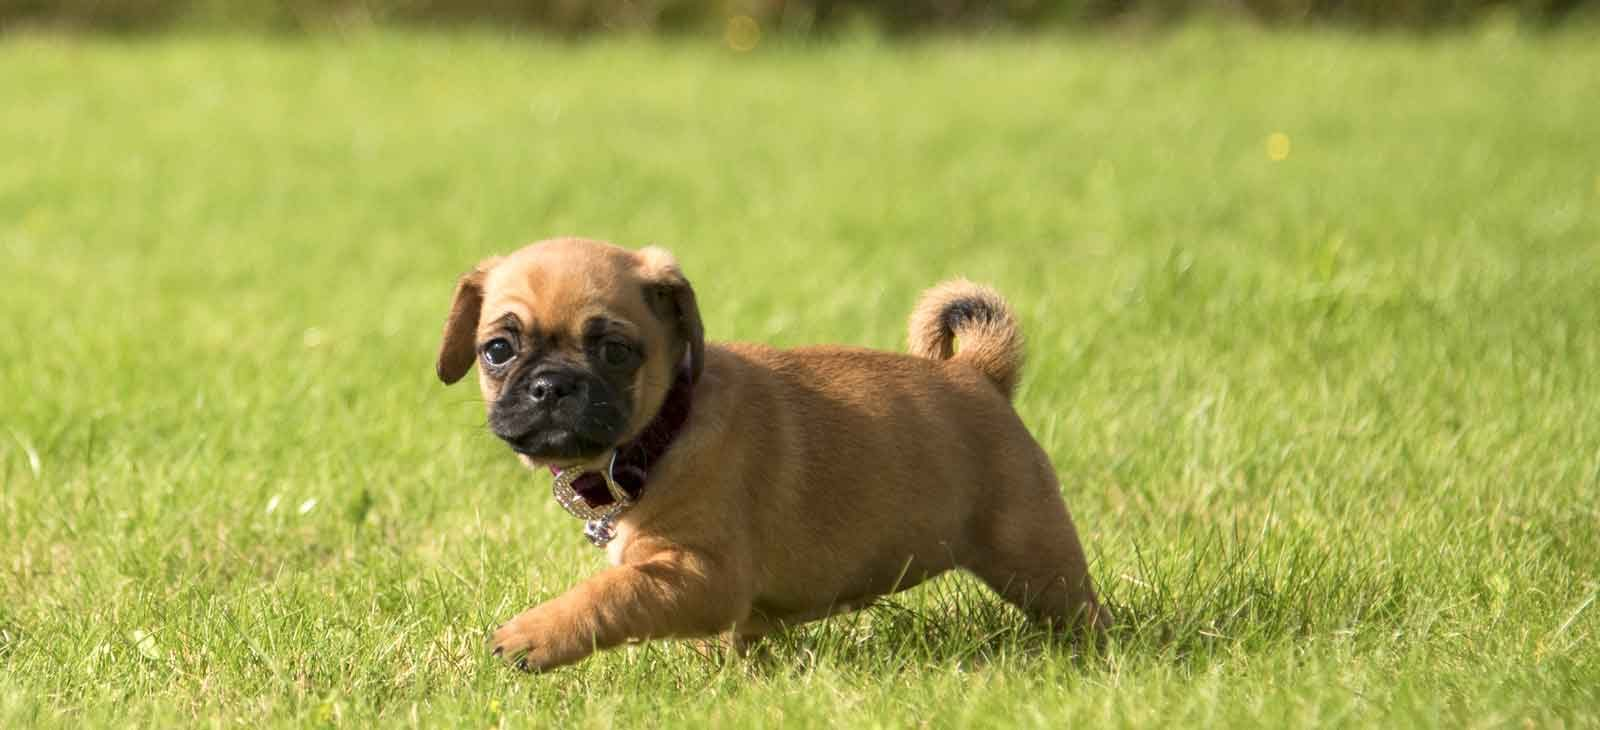
\includegraphics[scale=0.15]{puppy}}
\caption{Computer vision is interested in answering questions such as \textit{Is there a puppy in the image?} or \textit{Where is the puppy in the image?}}
\end{figure}

There are many sub-fields of computer vision such as scene reconstruction, event detection, video tracking, object recognition, 3D pose estimation, and motion estimation. This paper will focus on classification, using an approach called semantic segmentation. Shelhamer, Long and Darrell (2016) define semantic segmentation as a method of inference which is able to categorise fine image details. This is achieved by classifying each pixel in the image, and labelling it with the class of its enclosing object or region. A Fully Convolutional Neural Network (FCN) is proposed as the architecture to implement semantic segmentation. An FCN model was trained and implemented on a robotic agent.

\begin{figure}[h]
\begin{minipage}{0.45\textwidth}
\centering
\frame{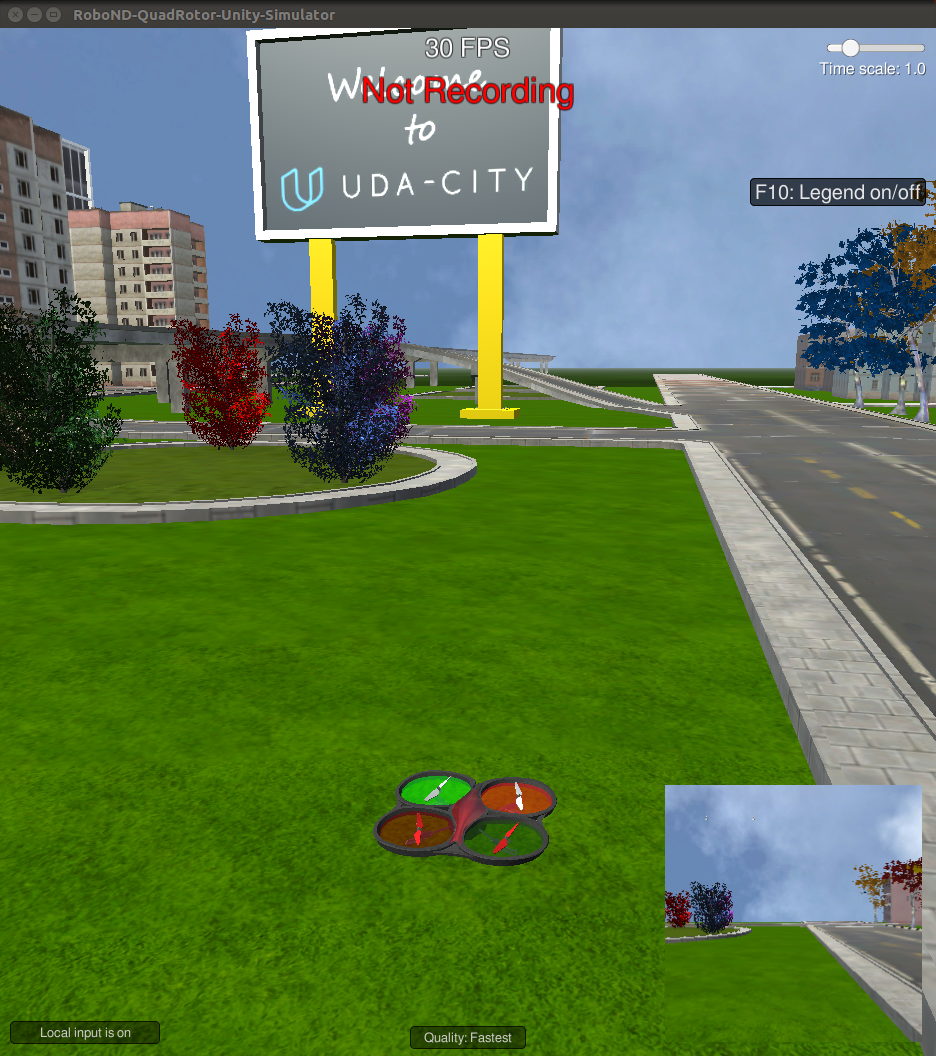
\includegraphics[height=6cm]{agent_image}}
\caption{The UAV agent in the simulated environment.}
\end{minipage}
\hspace{1cm}
\begin{minipage}{0.45\textwidth}
\centering
\frame{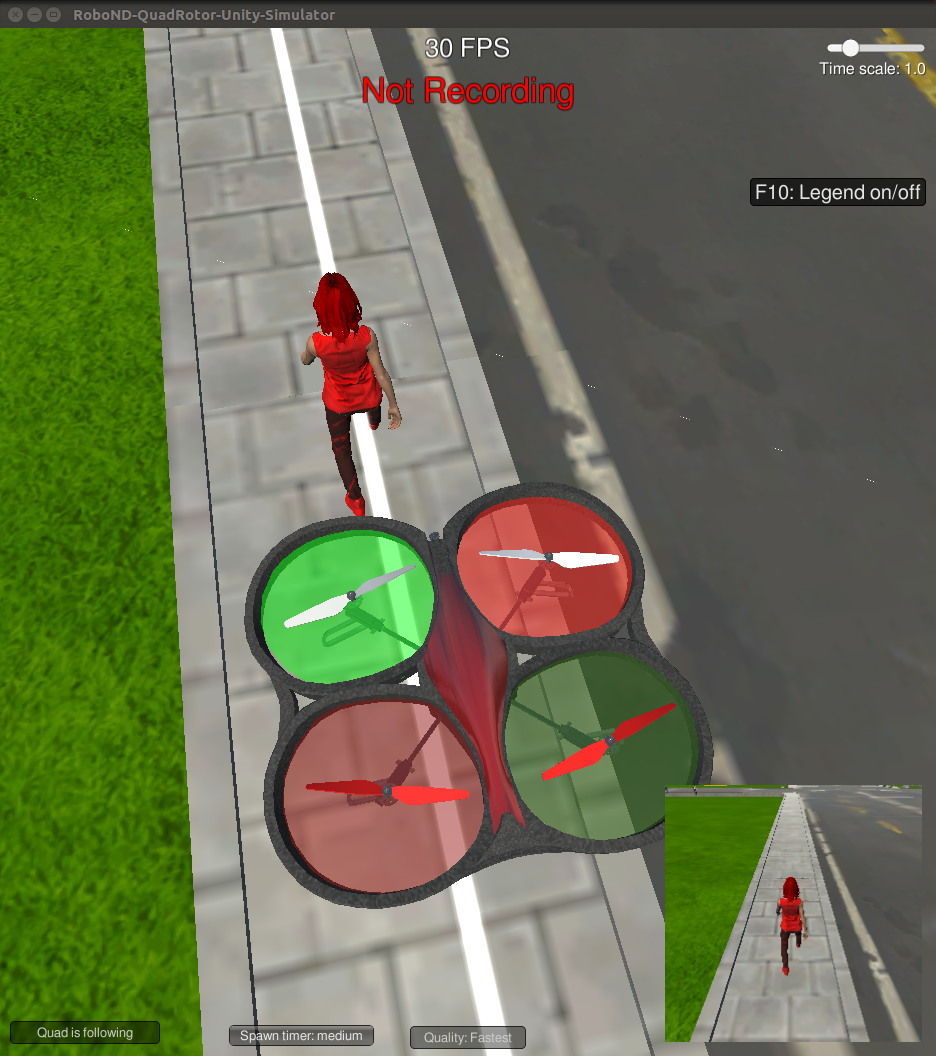
\includegraphics[height=6cm]{hero_image}}
\caption{The \textit{hero} can be seen coloured in red, with the UAV agent following her.}
\end{minipage}
\end{figure}

The agent was tasked with the identification (and subsequent tracking) of an individual, known as the \textit{hero}, in a 3D simulated environment built with Unity. The 3D simulated environment is a small city consisting of buildings, roads, elevated highways, and vegetation. The robotic agent is an unmanned aerial vehicle (UAV), as shown in Figure 2, which is fitted with a panning optical camera. The agent roams the simulation until it is able to locate the hero using the trained FCN, at which point the UAV will track the hero. The hero is a simulated person, as seen in Figure 3. To satisfy the assignment criteria, the proposed FCN model must achieve above a 40\% benchmark for an intersection over union metric. 

\section{Network Architecture}
FCNs are widely used for computer vision applications, and are a type of Artificial Neural Network (ANN). ANNs are computational models which, once trained on a dataset, can be used to make classification predictions, or  value estimations, based on a set of feature inputs that the model has been trained on. A typical fully connected feed-forward ANN consists of an input layer, one or more hidden layers, and an output layer, as shown in Figure 4. Hidden layers are made up of multiple nodes. The nodes themselves contain a non-linear activation function, such as a sigmoid or ReLU, and receive weighted input from the previous layers in the model. The inputs from the previous layer, and the non-linear activation of a node form a computational element called a neuron (also known as a perceptron) - these can be loosely thought of as decision making elements. An example of a neuron can seen in Figure 5.
\begin{figure}[h]
\begin{minipage}{0.45\textwidth}
\centering
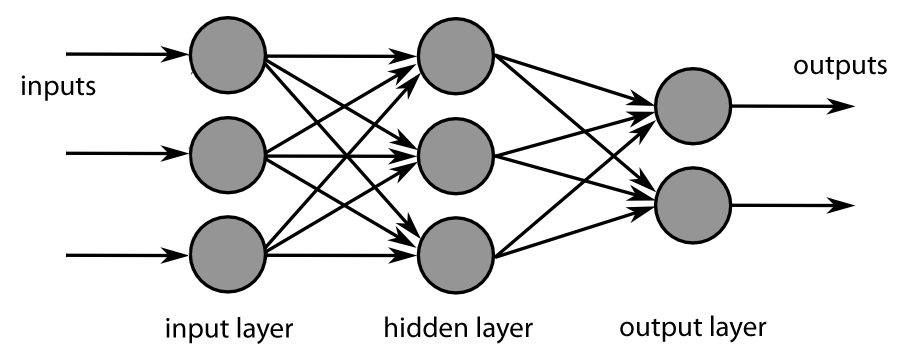
\includegraphics[scale=0.25]{feed_forward_neural_net}
\caption{A feed-forward artificial neural network consists of an input layer, which receives feature inputs, some hidden layers, and an output layer for classification.}
\end{minipage}
\hspace{1cm}
\begin{minipage}{0.45\textwidth}
\centering
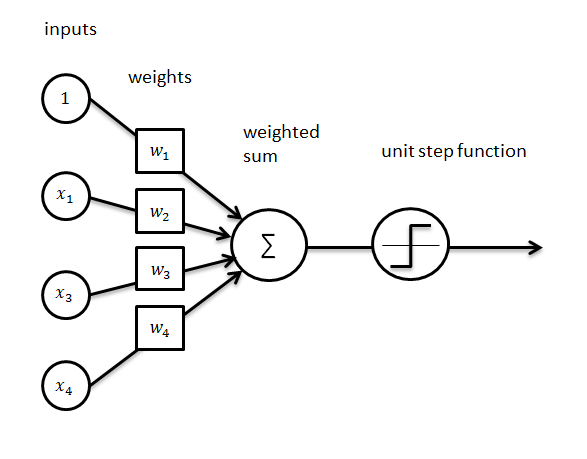
\includegraphics[scale=0.55]{perceptron}
\caption{The structure of a neuron (perceptron) includes weighted inputs from the previous layer, and a non-linear activation function.}
\end{minipage}
\end{figure}

Changing the weights in a neuron changes the neurons's contribution to the model, which in turn affects the overall model output. Weight changes occur during model training, which uses large volumes of labelled data to adjust the weights. Hidden layers are important because they allow highly non-linear models to be constructed, providing an approach for estimating complex phenomena which may be difficult to model with classical approaches, or computationally intractable. Generally, the more hidden layers, the more non-linear the model. Network architectures with multiple hidden layers have become so wide spread that the term Deep Neural Network (DNN) was coined to describe feed-forward ANNs which use two or more hidden layers. It must be noted that whilst increased non-linearity may allow us to model more complex phenomenon, making the ANN deeper does not guarantee increased model performance. This is mainly due to the fact that deeper models may over-fit the data during training, resulting in a failure to generalise on test and validation data sets.  

\begin{table}[h]
\centering
\caption{Reproduced from Ciresan, Meier, Gambardella, and Schmidhuber (2010) - DNN architectures of varying size for classifying the MNIST data set, and the associated performance of each network.} \footnotesize
\begin{tabular}{lS[table-format=3.2]S[table-format=3.2]S[table-format=3.2]S[table-format=3.2]}
\toprule
{\textbf{Architecture}} & {\textbf{Test Error}} & {\textbf{Best Test}} & {\textbf{Simulation}} & {\textbf{Weights}}\\
{\textbf{(number of neurons in each layer)}} & {\textbf{Best Validation [\%]}} & {\textbf{Error [\%]}} & {\textbf{Time [min]}} & {\textbf{[Millions]}}\\
\midrule
1000, 500, 10 & 0.49 & 0.44 & 23.4 & 1.34\\
1500, 1000, 500, 10 & 0.46 & 0.40 & 44.2 & 3.26\\
2000, 1500, 1000, 500, 10 & 0.41 & 0.39 & 66.7 & 6.69\\
2500, 2000, 1500, 1000, 500, 10 & 0.35 & 0.32 & 114.5 & 12.11\\
9 $\times$ 1000, 10 & 0.44 & 0.43 & 107.7 & 8.86\\
\bottomrule
\end{tabular}
\end{table}

Fully connected feed-forward DNNs have proven effective in computer vision classification problems, such as optical character recognition. One of the most widely cited examples of this is a feed-forward DNN performing classification on the MNIST dataset. The MNIST dataset contains handwritten digits, from 0 to 9, and is considered a benchmark for measuring neural net classification performance for the optical character recognition problem. Table 1, taken from paper by Ciresan, Meier, Gambardella, and Schmidhuber (2010), shows a table of feed-forward DNNs with varying numbers of hidden layers, and hidden layer depth.

\vspace{0.5cm}

\begin{minipage}{0.45\textwidth}
Notably, every model listed presents an error rate of less than 1\%. Generally, the deeper a network, the better the model's predictive performance, although this is not always the case as previously outlined. Figure 5, taken from the same paper, shows a small set of the misclassified images. Despite the misclassification it can be seen that, in most cases, the handwritten digit bears a high resemblance to the predicted value, and that the second prediction is generally correct. Remarkably, DNNs are not considered state of the art for image classification problems - even with simple tasks like MNIST classification. This is due to model inefficiencies that arise from image variation in the spatial domain.
\end{minipage}
\hspace{1cm}
\begin{minipage}{0.45\textwidth}
\centering
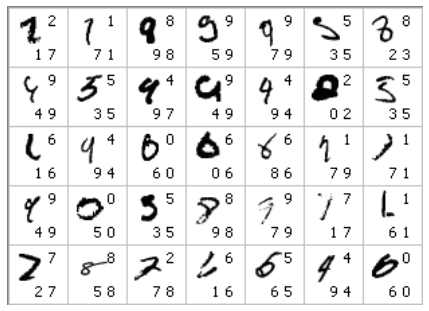
\includegraphics[height=3.5cm]{misclassification}
\captionof{figure}{Misclassified hand written digits by the top performing DNN from Ciresan, Meier, Gambardella, and Schmidhuber (2010). The digit in the top right hand corner of the box is the observation label, and the two digits in the bottom right hand corner are the predictions from the DNN model.}
\end{minipage}

\vspace{0.5cm}

The problem can be better understood by considering Figures 7 and 8. Figure 7 shows an image with a puppy on the left, and Figure shows an image with a puppy on the right. Suppose we create a simple model to classify whether an image has a puppy in it or not, and assume we train this model with lots of images like the one shown in Figure 7. If the trained model was then used to classify images like the one shown in Figure 8 it would perform poorly. This is because our model would have only learned to classify pixel features on the left side of the picture with puppies, which says nothing about identifying a puppy on the right hand side of an image. Put simply, there is no \textit{translational invariance} in the model.

\vspace{0.25cm}

\begin{figure}[h]
\begin{minipage}{0.45\textwidth}
\centering
\frame{
\includegraphics[height=4cm]{doggo_left}}
\caption{An image in which a puppy is located on the left hand side of the image.}
\end{minipage}
\hspace{1cm}
\begin{minipage}{0.45\textwidth}
\centering
\frame{
\includegraphics[height=4cm]{doggo_right}}
\caption{An image in which a puppy is located on the right hand side of the image.}
\end{minipage}
\end{figure}

\newpage

\subsection{Convolutional Neural Networks}
A Convolutional Neural Network (CNN) is a class of ANN, which has an underlying network structure which is better at learning shapes, edges, and colours meaning it is less reliant on the spatial location of a classification object in an image. Recall that vanilla feed-forward neural nets only have neuron connections from the previous layer, and there are no connections from neurons in the same layer - weights are not shared. In contrast, CNNs share neuron weights by using filters which are convolved over an input image. Consider a raw input image of say 32 $\times$ 32 pixels, with a depth of 3 colour channels, as shown in Figure 9.
\begin{figure}[h]
\begin{minipage}{0.45\textwidth}
\centering
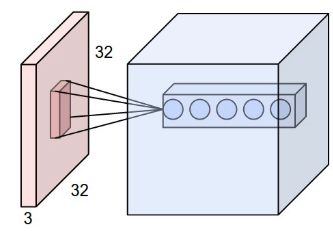
\includegraphics[scale=0.4]{CNN}
\caption{The raw image input is 32 $\times$ 32, with a 3-channel depth (R,G,B). The filter is a 3 $\times$ 3 patch with the same depth as the input. The filter is convolved over the image using some stride - each convolution creates a single element output which forms part of the 2D activation map (i.e. the output). There are $K$ filters convolved over the image, a parameter chosen as part of the architecture, and the output volume represents the stacked 2D activation maps.}
\vspace{0.5cm}
\end{minipage}
\hspace{1cm}
\begin{minipage}{0.45\textwidth}
\centering
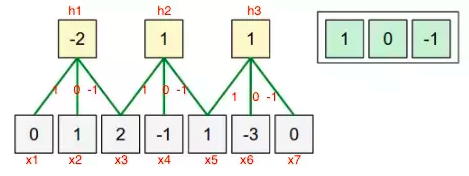
\includegraphics[scale=0.43]{CNN_example}
\caption{An simple example of weight sharing that takes place in a CNN. The white 1D array represents the input image, and the blue 1D array represents the filter. The filter (blue) is convolved across the input (white) using a stride of 2. The convolved output, which represents the activation map, can be seen in yellow. This architecture allows for the sharing of the weights in the model.}
\end{minipage}
\end{figure}

The convolving filter, which contains the model weights, is the small patch which is incident on the raw input image surface. The image section in contact with the filter is called the receptive field - this changes as the filter convolves an image. Filter width and height are parameters chosen as part of the network architecture, and filter depth is identical to the input image depth. The filter is moved around the image according to the number of pixels in each stride. After each movement, the filter weights are multiplied by the receptive field and added together - this makes up a single entry in the 2D activation map which forms part of the output volume. The width and height of the output volume are dependent on the stride, and the type of padding used during the convolution. Finally, the output depth is dependent on the number of filters specified in the network architecture - typically this parameter is denoted as $K$. The output volume is simply the stacked 2D activation maps from each filter. It is the convolutional process, whereby the filter weights are used over an entire image, that provide the weight sharing seen in CNNs. Figure 10 provides a simple example of how this works. In this example, the filter is a 1D array (shown in blue), and the input image is also a 1D array (shown in white). The filter (blue) is convolved over the input image (white) with a stride of 2. The filter weights are multiplied with the image values, and added together to form the output volume - a 1D array (shown in yellow).\\

CNNs provide superior performance over DNNs in the image classification domain. This was demonstrated on the MNIST dataset by LeCun (1998) with his LeNet (pictured in Figure 11), and again by Krizhevsky (2012) on the ImageNet dataset with AlexNet (shown in Figure 12). Whilst CNNs can achieve noteworthy performance in the task of image classification, there is a notable performance loss when they are re-tasked with pixel by pixel classification known as semantic segmentation. This is due to the fact that fully connected layers don't preserve spatial information.
\begin{figure}[h]
\centering
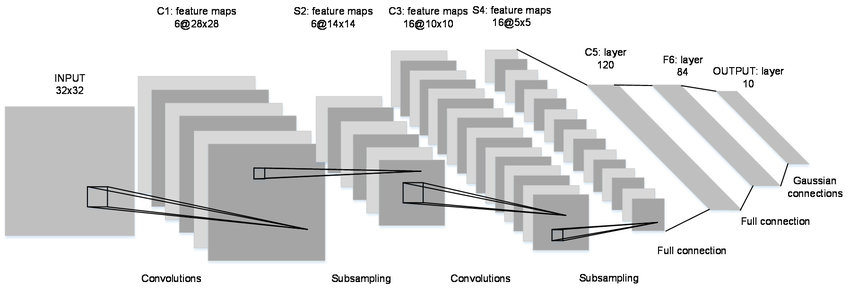
\includegraphics[scale=0.6]{lenet5}
\caption{The architecture of a CNN called LeNet5, taken from the Lecun (1998), used to classify the MNIST data set.}
\end{figure}

\begin{figure}[h]
\centering
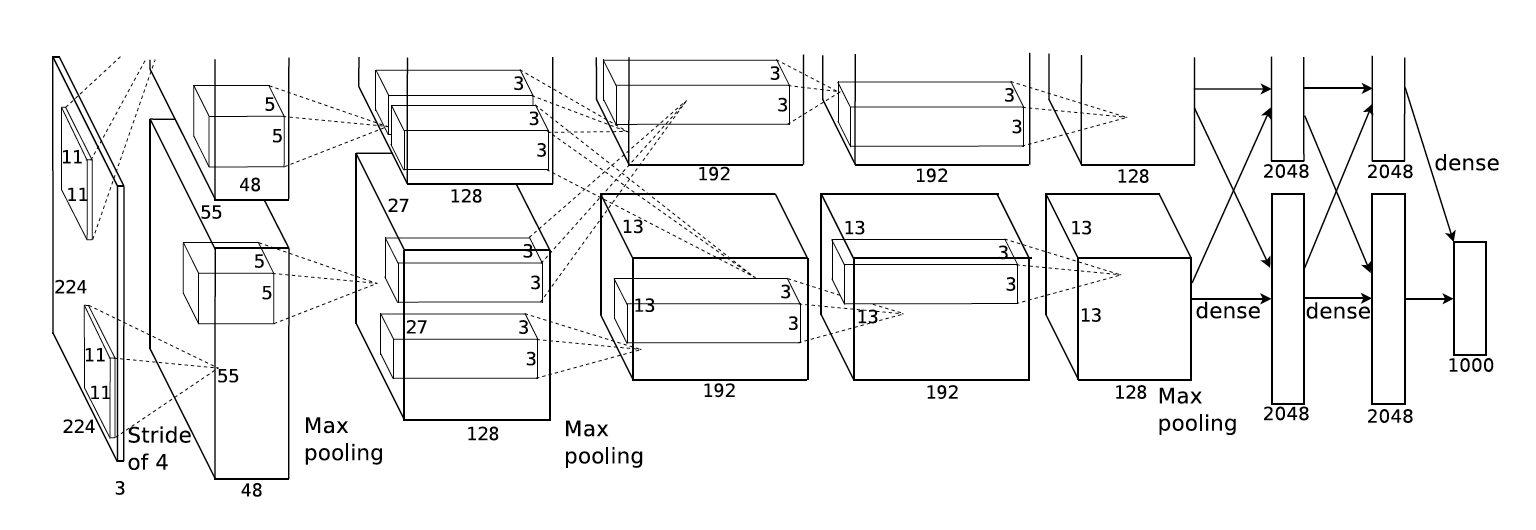
\includegraphics[scale=0.25]{alexnet}
\caption{The architecture of a CNN called Alexnet, taken from Krizhevsky (2012), used to classify the image database called ImageNet.}
\end{figure}

\clearpage

\subsection{Fully Convolutional Neural Networks}
FCNs preserve spatial information, and represent a state-of-the-art approach to semantic segmentation. Structurally, they can be thought of as two distinct parts: encoders and decoders. This is shown in Figure 13. The encoder is comprised of several convolutional layers, which are typically arranged to progressively concentrate the spatial domain, and increase the number of channels in the image. These different layers of spatial compression are useful for training the model on different image resolutions. The decoder, in contrast, upsamples encoder compressions, restoring the spatial information to the output - typically the final layer restores the output to the initial input image dimensions, before being passed to a convolutional layer with a softmax activation function.
\vspace{0.25cm}
\begin{figure}[h]
\centering
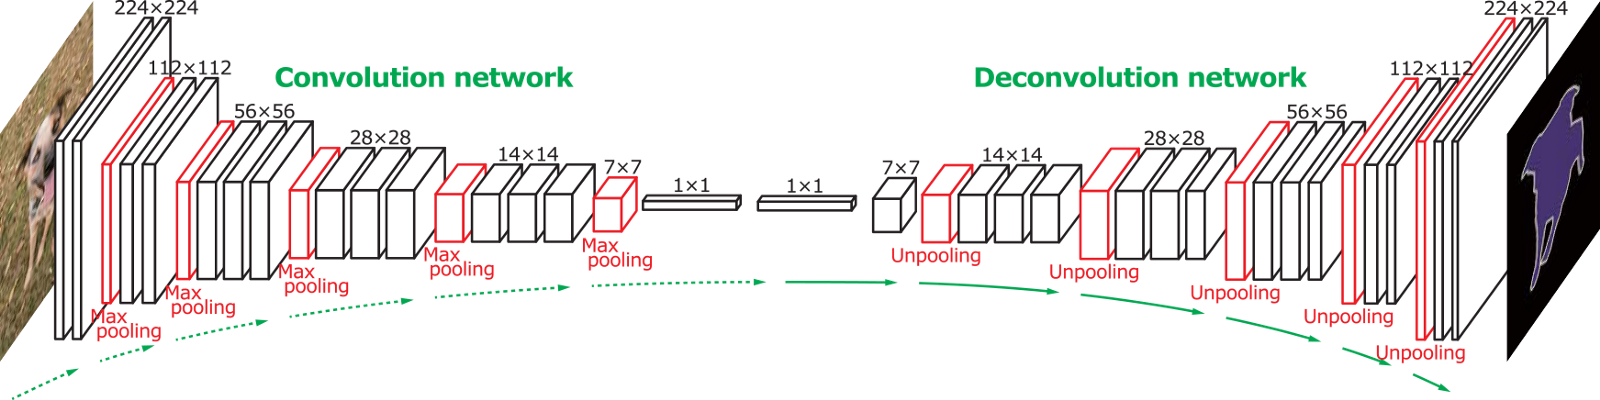
\includegraphics[scale=0.25]{FCN}
\caption{Structurally FCNs can be thought of as an encoder (convolutional network) connected to a decoder (deconvolutional network)}
\end{figure}

FCNs are often make use of 1 $\times$ 1 convolutions, which are just a 2D convolution of patch size 1 $\times$ 1, and a stride of 1 (Lin, Chen, \& Yan, 2014). The spatial dimensions of the convolved image are preserved in the output volume, but the desired number of filters ($K$) changes the output volume depth. Indeed this is one of the main incentives to use 1 $\times$ 1 convolutions - they are computationally cheap, and can reduce the image depth making subsequent operations less expensive. One approach that has been used is to intersperse convolutional layers with 1 $\times$ 1 convolutional layers, to reduce the depth of the image being convolved by larger patches (e.g. 3 $\times$ 3, or 5 $\times$ 5). An example of this can be seen in Figure 14. Of course, this is not the only way that 1 $\times$ 1 convolutional layers can be used. They can also be used to add more depth to a model, and additional non-linearity since the 1 $times$ 1 layer contains an activation function like ReLU. Using 1 $\times$ 1 convolutions is considered a cheap way of doing this.  
\begin{figure}[h]
\centering
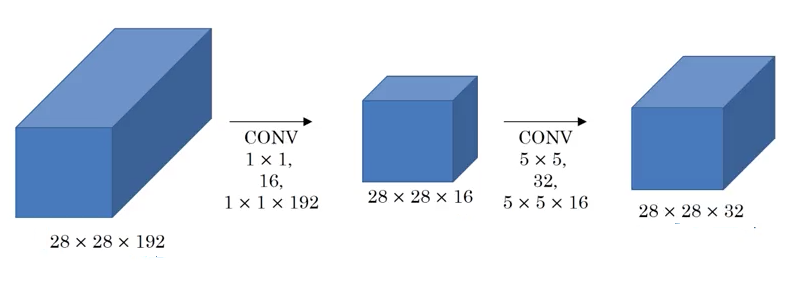
\includegraphics[scale=0.4]{1by1}
\caption{The input is 28 $\times$ 28 $\times$ 192 and the desired 2D convolution is a 5 $\times$ 5 patch using 32 filters. This would result in a total of XXXX multiplications. If a 1 $\times$ 1 convolution is used to reduce the depth of the input image from 192 to 16 before performing the 2D convolution with the 5$\times$5 patch, this reduces the total number of multiplications to XXXX.}
\end{figure}

Finally, FCNs see an improvement in model performance with the use of something called skip connections. A skip connection attaches a residual output in an FCN architecture to an output occurring later in the network. Their use was originally proposed by He, Zhang, Ren and Sun (2015) who found that adding more layers to their model \textit{worsened} the performance during training. This work led to the development of the well known Resnet architecture. The skip connections essentially concatenate the 2 layers by adding the outputs - an example of the operation can be seen in Figure 15.
\begin{figure}[h]
\centering
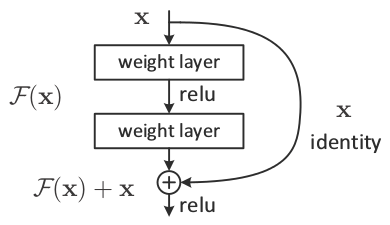
\includegraphics[scale=0.5]{skip}
\caption{An example of a skip connection - the residual output in the network literally skips a section of the network and is concatenated with a later output of the model.}
\end{figure}

\subsection{Proposed Architectures \& Implementation}
The information presented so far makes a compelling case for the use of FCNs to perform the semantic segmentation task, however, there is some uncertainty as to what model architecture should be employed. State of the art FCNs involve multiple 2D convolution layers interspersed with pooling layers in the encoder. The decoder consists of up-sampling layers interspersed with un-pooling layers. Additionally, these state of the art networks make use of 1 $\times$ 1 convolutions, and skip connections.An example of this can be seen in Figure 16, which shows an FCN network called SegNet taken from a paper by Badrinarayanan, Kendall, and Cipolla (2016).
\begin{figure}[h]
\centering
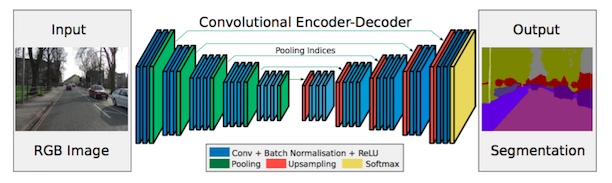
\includegraphics[scale=0.6]{segnet}
\caption{An example of a fully convolutional network with pooling, upsampling, and skip connections}
\end{figure}

FCN networks with many layers, like the original FCN architecture by Shelhamer, Long, and Darrell (2014) and SegNet, are used to provide semantic segmentation on images with high visual complexity taken from the real world. In contrast, the models proposed in this paper are tasked with semantic segmentation of images taken from the 3D environment simulated in Unity. Given this, it may not be appropriate to adopt the depth seen in state-of-the-art FCN architectures since reasonable performance may be achieved with smaller models. Moreover, given that the dataset from the simulation only consists of approximately 4000 images (about half of the 9,993 found in the VOC2012 segmentation data set), a more complex model may result in worse performance. In this light, three different FCN architectures are proposed for investigation: a deep model with 1 $\times$ 1 convolutions; a shallow model with 1 $\times$ 1 convolutions; and a shallow model without 1 $\times$ 1 convolutions. These models are discussed in more detail in Sections 2.3.2, 2.3.3, and 2.3.4 respectively. 

\subsubsection{Tensorflow Implementation}
To make the model implementation easier, two functions were developed: \verb|encoder_block()| (shown in Listing 1), and \verb|decoder_block()| (shown in Listing 2). An interesting feature of the \verb|encoder_block()| is that it uses the a seperable 2D convolution. The reason for this is that separable convolutions are more computationally efficient. To see this, consider a 3 $\times$ 3 patch with one filter ($K = 1$) in a single convolution. The number of operations to perform this is XXXX. A matrix is seperable if it can be written as follows:
\begin{align}
\begin{bmatrix}
A \cdot a & A \cdot b & A \cdot c\\
B \cdot a & B \cdot b & B \cdot c\\
C \cdot a & C \cdot b & C \cdot c
\end{bmatrix}
=
\begin{bmatrix}
A\\
B\\
C
\end{bmatrix}
\cdot
\begin{bmatrix}
a & b & c
\end{bmatrix}
\end{align}  

The definition shown in (1) can be used to first undertake a convolution with XXXX, and then convolve the result of the first convolution with XXXX. This results in a total of XXXX operations. Given that FCNs have to perform this type of operation many times to convolve an entire image, there are significant computational savings made by using separable 2D convolutions.
   
\begin{figure}[h]\scriptsize
\begin{sexylisting}{Implementation of the encoder block for the FCN in TensorFlow}
def encoder_block(input_layer, filters, strides):
    
    # TODO Create a separable convolution layer using the separable_conv2d_batchnorm() function.
    output_layer = separable_conv2d_batchnorm(input_layer, filters, strides)
    
    return output_layer
\end{sexylisting}
\end{figure}

The \verb|decoder_block()| function takes three arguements, two of them being layers. The smallest input layer is upsampled using the \verb|bilinear_upsample()| function - this simply doubles the size of the small layer, and fills the additional spaces with copies of the small layer rows and columns. The second layer input is a skip connection which comes from the encoder of the FCN. The upsampled layer and the layer from the skip connection are added together using a concatenate function. Note that care must be taken to ensure there is no mismatch in the layer dimensions. The concatenated layers are then passed through a 2D convolution to create the final layer.  

\begin{figure}[h]\scriptsize
\begin{sexylisting}{Implementation of the decoder block for the FCN in TensorFlow}
def decoder_block(small_ip_layer, large_ip_layer, filters):
    
    # TODO Upsample the small input layer using the bilinear_upsample() function.
    small_ip_upsample = bilinear_upsample(small_ip_layer)
    
    # TODO Concatenate the upsampled and large input layers using layers.concatenate
    concat_layer = layers.concatenate([small_ip_upsample, large_ip_layer])
    
    # TODO Add some number of separable convolution layers
    output_layer = separable_conv2d_batchnorm(concat_layer, filters)
    
    return output_layer
\end{sexylisting}
\end{figure}

Both the \verb|encoder_block()| and \verb|decoder_block()| functions use ReLUs as the non-linear activation functions, and both functions employ batch normalisation. Batch normalisation is a technique proposed by Ioffe and Szegedy (2015) which helps to improve the optimisation process which occurs during training. Additionally, it provides some regularisation to the model as well.

\clearpage

\subsubsection{Model 1: Deep Model with 1 $\times$ 1 Convolution}
The proposed deep model with 1 $\times$ 1 convolutions is comprised of 9 layers, including the input layer - the network architecture can be seen in Figure 17, and a detailed description of each layer can be found in Table 2.
\begin{figure}[h]
\centering
\begin{tikzpicture}[scale=0.83, every node/.style={scale=0.83}]
\newcommand*\circled[1]{\tikz[baseline=(char.base)]{
            \node[shape=circle,draw,inner sep=2pt] (char) {#1};}}
            
    \node[anchor=south west,inner sep=0] (image) at (0,0) {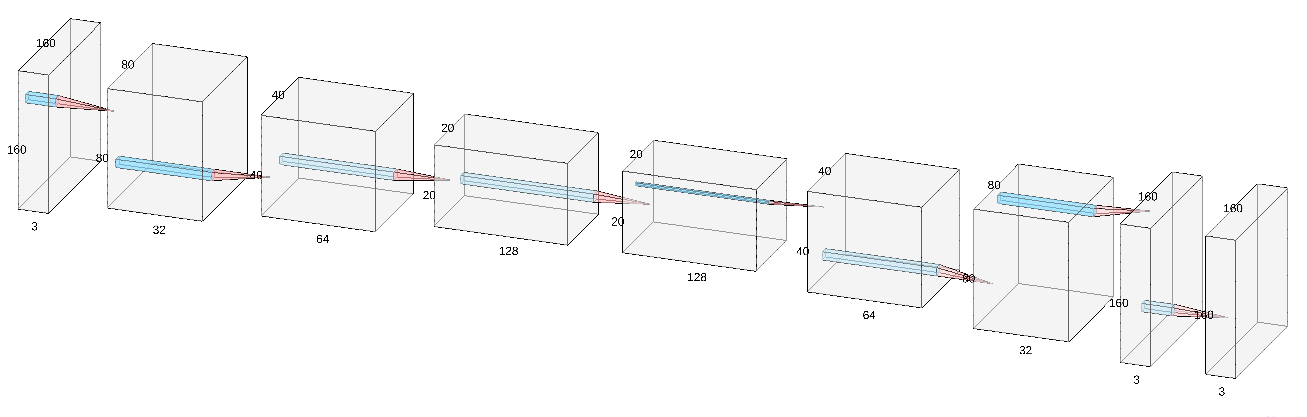
\includegraphics[scale=0.33]{model_3(1_paper)}};
    
    \node[] at (1.8,1) {\circled{1}};
    \node[] at (3.8,0.718) {\circled{2}};
    \node[] at (5.8,0.437) {\circled{3}};
    \node[] at (8,0.1291) {\circled{4}};
    \node[] at (10.2,-0.1795) {\circled{5}};
    \node[] at (12,-0.4322) {\circled{6}};
    \node[] at (13.2,-0.6) {\circled{7}};
    
    \draw[->, >=stealth] (4,4) to [out=20,in=120] (10.2,3.2);
    \draw[->, >=stealth] (2.2,4.5) to [out=20,in=120] (12,3.1);
    \draw[->, >=stealth] (1,4.8) to [out=20,in=120] (13.8,3);
\end{tikzpicture}
\caption{Graphical depiction of model 1}
\end{figure}

\begin{table}[h]
\centering
\caption{Detailed breakdown of the structure for model 1}\scriptsize
\begin{tabular}{ccccp{8cm}}
\toprule
\textbf{Name} & \textbf{Width (W)} & \textbf{Height (W)} & \textbf{Depth (D)} & Layer Details\\  
\midrule
 & & & &\\
Input & 160 & 160 & 3 & Raw image input\\
 & & & &\\
1 & 80 & 80 & 32 & Created from 2D convolution of raw image input with 32 filters of patch size 3 $\times $ 3, and the stride is 2 with same padding\\
 & & & &\\
2 & 40 & 40 & 64 & Created from 2D convolution of layer 1 with 64 filters of patch size 3 $\times $ 3, and the stride is 2 with same padding\\
 & & & &\\
3 & 20 & 20 & 128 & Created from 2D convolution of layer 2 with 128 filters of patch size 3 $\times$ 3, and the stride is 2 with same padding\\
 & & & &\\
4 & 20 & 20 & 128 & Created from 2D convolution of layer 3 with 128 filters of patch size 1 $\times$ 1, and the stride is 1 with same padding\\
 & & & &\\
5 & 40 & 40 & 64 & Created by adding upsampled layer 4 to layer 2 with a skip connection, and passed through a 2D convolution with 64 filters of patch size 3 $\times$ 3 and stride XXXX\\
 & & & &\\
6 & 80 & 80 & 32 & Created by adding upsampled layer 5 to layer 1 with a skip connection, and passed through a 2D convolution with 32 filters of patch size 3 $\times$ 3 and stride XXXX\\
 & & & &\\
7 & 160 & 160 & 3 & Created by adding upsampled layer 6 to the inputs with a skip connection, and passed through a 2D convolution with 3 filters of patch size 3 $\times$ 3 and stride XXXX\\
& & & &\\
Output & 160 & 160 & 3 & Created from a 2D convolution\\
\bottomrule
\end{tabular}
\end{table}

\newpage

\subsubsection{Model 2: Shallow Model with 1 $\times$ 1 Convolution}
The proposed deep model with 1 $\times$ 1 convolutions is comprised of 9 layers, including the input layer - the network architecture can be seen in Figure 18, and a detailed description of each layer can be found in Table 3.
\begin{figure}[h]
\centering
\begin{tikzpicture}
\newcommand*\circled[1]{\tikz[baseline=(char.base)]{
            \node[shape=circle,draw,inner sep=2pt] (char) {#1};}}
            
    \node[anchor=south west,inner sep=0] (image) at (0,0) {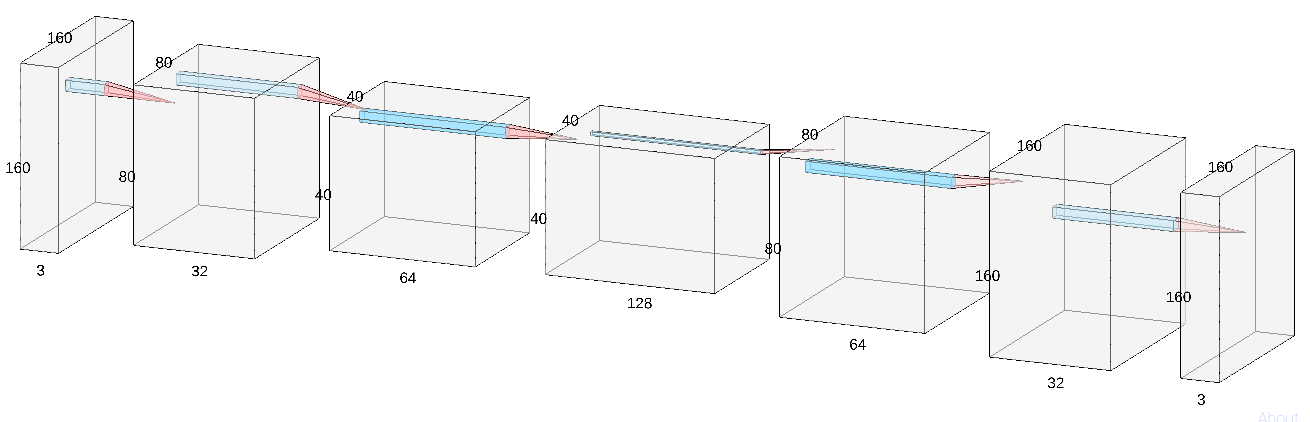
\includegraphics[scale=0.33]{model_2(2_paper)}};
    
        \node[] at (2.3,1) {\circled{1}};
        \node[] at (4.8,0.7) {\circled{2}};
        \node[] at (7.3,0.4) {\circled{3}};
        \node[] at (9.8,0.1) {\circled{4}};
        \node[] at (12.3,-0.2) {\circled{5}};
	    
	    \draw[->, >=stealth] (2.8,4.5) to [out=20,in=120] (10.5,3.8);
	    \draw[->, >=stealth] (1.3,4.9) to [out=20,in=120] (13,3.6);
	    
\end{tikzpicture}
\caption{Graphical depiction of model 2}
\end{figure}

\begin{table}[h]
\centering
\caption{Detailed breakdown of the structure for model 2}\scriptsize
\begin{tabular}{ccccp{8cm}}
\toprule
\textbf{Name} & \textbf{Width (W)} & \textbf{Height (W)} & \textbf{Depth (D)} & Layer Details\\  
\midrule
 & & & &\\
Input & 160 & 160 & 3 & Raw image input\\
 & & & &\\
1 & 80 & 80 & 32 & Created from 2D convolution of raw image input with 32 filters of patch size 3 $\times $ 3, and the stride is 2 with same padding\\
 & & & &\\
2 & 40 & 40 & 64 & Created from 2D convolution of layer 1 with 64 filters of patch size 3 $\times $ 3, and the stride is 2 with same padding\\
 & & & &\\
3 & 40 & 40 & 128 & Created from 2D convolution of layer 2 with 128 filters of patch size 1 $\times$ 3, and the stride is 1 with same padding\\
 & & & &\\
4 & 80 & 80 & 64 & Created by adding upsampled layer 3 to layer 1 with a skip connection, and passed through a 2D convolution with 64 filters of patch size 3 $\times$ 3\\
 & & & &\\
5 & 160 & 160 & 32 & Created by adding upsampled layer 4 to the raw input with a skip connection, and passed through a 2D convolution with 32 filters of patch size 3 $\times$ 3\\
 & & & &\\
Output & 160 & 160 & 3 & Created from a 2D convolution\\
\bottomrule
\end{tabular}
\end{table}

\newpage

\subsubsection{Model 3: Shallow Model without 1 $\times$ 1 Convolution}
The proposed deep model with 1 $\times$ 1 convolutions is comprised of 8 layers, not including the input layer - the network architecture can be seen in Figure 19, and a detailed description of each layer can be found in Table 4.
\begin{figure}[h]
\centering
\begin{tikzpicture}
\newcommand*\circled[1]{\tikz[baseline=(char.base)]{
            \node[shape=circle,draw,inner sep=2pt] (char) {#1};}}
            
    \node[anchor=south west,inner sep=0] (image) at (0,0) 			{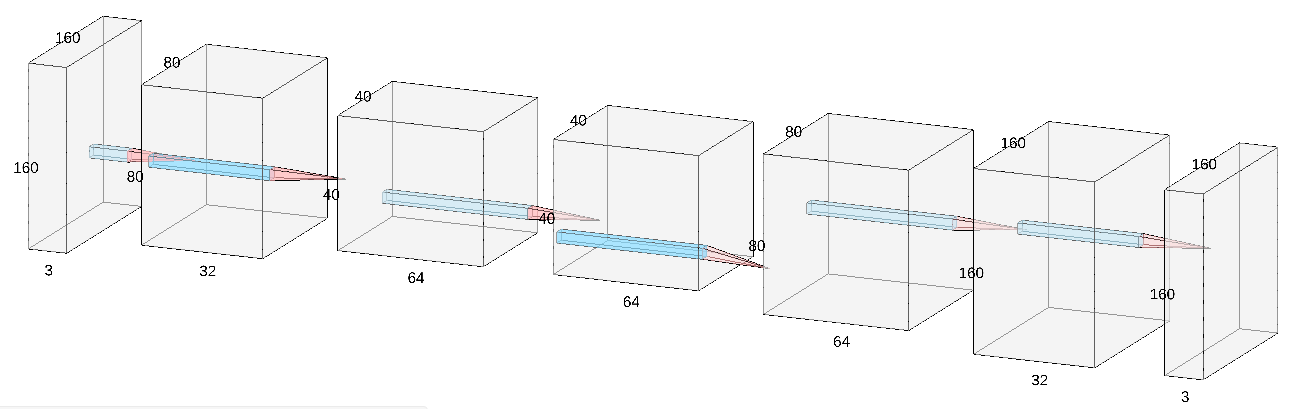
\includegraphics[scale=0.33]{model_1(3_paper)}};

    \node[] at (2.5,1) {\circled{1}};
    \node[] at (4.8,0.7183) {\circled{2}};
    \node[] at (7.3,0.4122) {\circled{3}};
    \node[] at (9.8,0.1061) {\circled{4}};
    \node[] at (12.3,-0.199) {\circled{5}};
    
    \draw[->, >=stealth] (3,4.3) to [out=20,in=120] (10.5,3.5);
	\draw[->, >=stealth] (1.3,4.7) to [out=20,in=120] (13,3.4);
\end{tikzpicture}
\caption{Graphical depiction of model 3}
\end{figure}

\begin{table}[h]
\centering
\caption{Detailed breakdown of the structure for model 3}\scriptsize
\begin{tabular}{ccccp{8cm}}
\toprule
\textbf{Name} & \textbf{Width (W)} & \textbf{Height (W)} & \textbf{Depth (D)} & Layer Details\\  
\midrule
 & & & &\\
Input & 160 & 160 & 3 & Raw image input\\
 & & & &\\
1 & 80 & 80 & 32 & Created from 2D convolution of raw image input with 32 filters of patch size 3 $\times $ 3, and the stride is 2 with same padding\\
 & & & &\\
2 & 40 & 40 & 64 & Created from 2D convolution of layer 1 with 64 filters of patch size 3 $\times $ 3, and the stride is 2 with same padding\\
 & & & &\\
3 & 40 & 40 & 64 & Created from 2D convolution of layer 2 with 64 filters of patch size 3 $\times$ 3, and the stride is 1 with same padding\\
 & & & &\\
4 & 80 & 80 & 64 & Created by adding upsampled layer 3 to layer 1 with a skip connection, and passed through a 2D convolution with 64 filters of patch size 3 $\times$ 3\\
 & & & &\\
5 & 160 & 160 & 32 & Created by adding upsampled layer 4 to raw inputs with a skip connection, and passed through a 2D convolution with 32 filters of patch size 3 $\times$ 3\\
& & & &\\
Output & 160 & 160 & 3 & Created from a 2D convolution\\
\bottomrule
\end{tabular}
\end{table}

\clearpage

\section{Data \& Network Training}
The initial data set provided with the problem was comprised of XXXX images. There are three rough categories that the images can be placed in:
\begin{enumerate}
\item Images while the UAV is following the \textit{hero}
\item Images while the UAV is patrolling, but cannot see the \textit{hero}
\item Images while the UAV is patrolling and can see the \textit{hero}
\end{enumerate}
To provide the network with additional training data, XXXX, XXXX, and XXXX images were captured from the simulator in each of the fields, respectively. These were added to the initial data set to bring it to a total of 5279 images. When an image is captured, pixel label data is also provided in the form of image masks. There are three types of masks that accompany each image: a mask highlighting the hero; a mask highlighting people who are not the hero; and a mask highlighting the background. Examples of these masks can be seen in Figures 20, 21, 22, and 23, respectively. It must be noted that these labels would not be available with real world images, and the masks are able to be extracted only because the image data is collected from a simulation.
\begin{figure}[h]
\begin{minipage}{0.45\textwidth}
\centering
\frame{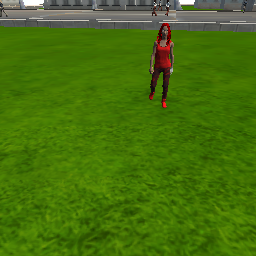
\includegraphics[height=4cm]{cam1}}
\captionof{figure}{An image captured from the simulation}
\end{minipage}
\hspace{1cm}
\begin{minipage}{0.45\textwidth}
\centering
\frame{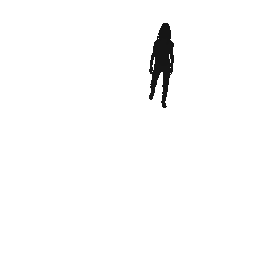
\includegraphics[height=4cm]{cam2}}
\captionof{figure}{A mask of the image seen in Figure 20 highlighting pixels which contain the \textit{hero}}
\end{minipage}
\end{figure}

\begin{figure}[h]
\begin{minipage}{0.45\textwidth}
\centering
\frame{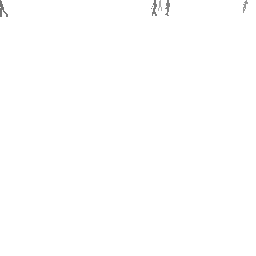
\includegraphics[height=4cm]{cam3}}
\captionof{figure}{A mask of the image seen in Figure 20 highlighting pixels which contain people other than the \textit{hero}}
\end{minipage}
\hspace{1cm}
\begin{minipage}{0.45\textwidth}
\centering
\frame{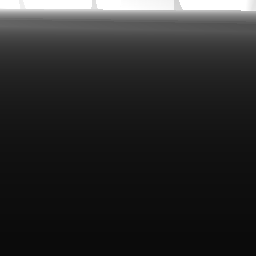
\includegraphics[height=4cm]{cam4}}
\captionof{figure}{A mask of the image seen in Figure 20 highlighting pixels which contain the background}
\end{minipage}
\end{figure}

Prior to model training, there is some pre-processing which concatenates the mask images into a single image. The network is trained using an optimiser called Adam, which is similar to Stochastic Gradient Descent (SGD). It differs in one important way: SGD typically uses a static learning rate, whereas Adam computes adaptive learning rates for each parameter (Ruder, 2017). Talk about the use of hyperparameters for training the network

\newpage

\subsection{Batch Size}
\begin{minipage}{0.45\textwidth}
Batch size defines the number of training samples/images propagated through the network in a single pass. Batch size has an upper bound dependent on the amount of RAM in the GPU - we cannot accommodate more images than can be stored in RAM for a pass. A small experiment was conducted to gain some intuition on how batch size affects model performance. Model performance was tested for a series of increasing batch sizes, setting learning rate at 0.01, number of epochs at 5, and number of steps per epoch to 80. Figure 24 shows the training loss for increasing batch size.
\end{minipage}
\hspace{1cm}
\begin{minipage}{0.45\textwidth}
\centering
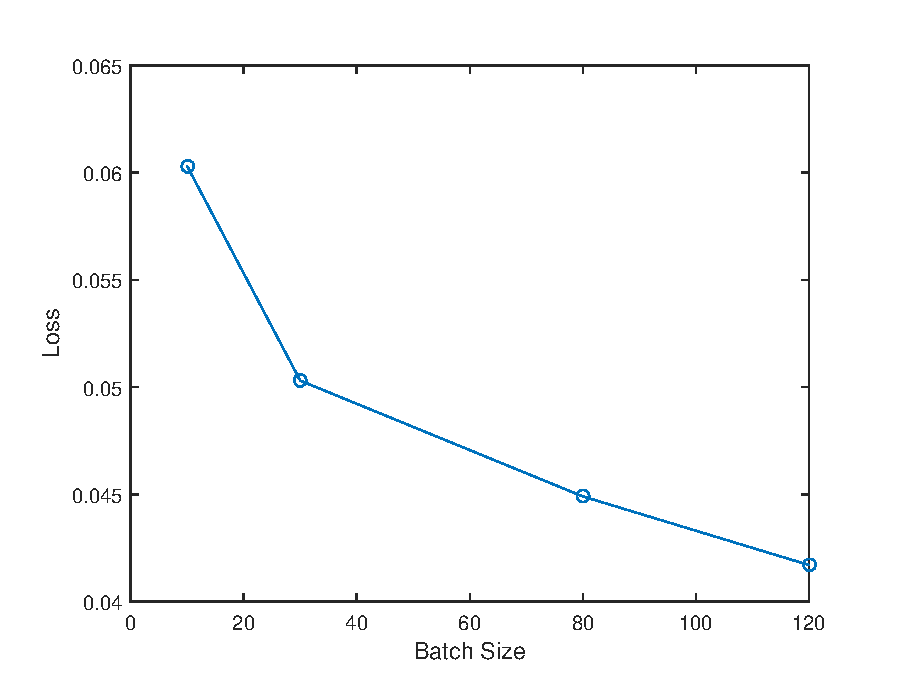
\includegraphics[height=4.7cm]{hyp_par_1}
\captionof{figure}{Change in loss function as batch size is increased}
\end{minipage}

\vspace{0.3cm}

Clearly increased batch size allows more training images to pass through the model resulting in better performance - which is in line with intuition. This relationship is most likely follows a law of diminishing returns, with increases in performance reaching some asymptotic limit as batch size increases further.

\subsection{Epochs}
\begin{minipage}{0.45\textwidth}
Epochs are the number of times the entire data set gets propagated through the network. Intuition would suggest that the more epochs, the more the model would be exposed to the training dataset, resulting in a better performance. Evidence supporting this intuition can be seen in Figure 25, which shows a small experiment in which the loss function was measured for an increasing number epochs. Note that the other model hyper-parameters were held constant with learning rate of 0.01, batch size 20, and number of steps 80.
\end{minipage}
\hspace{1cm}
\begin{minipage}{0.45\textwidth}
\centering
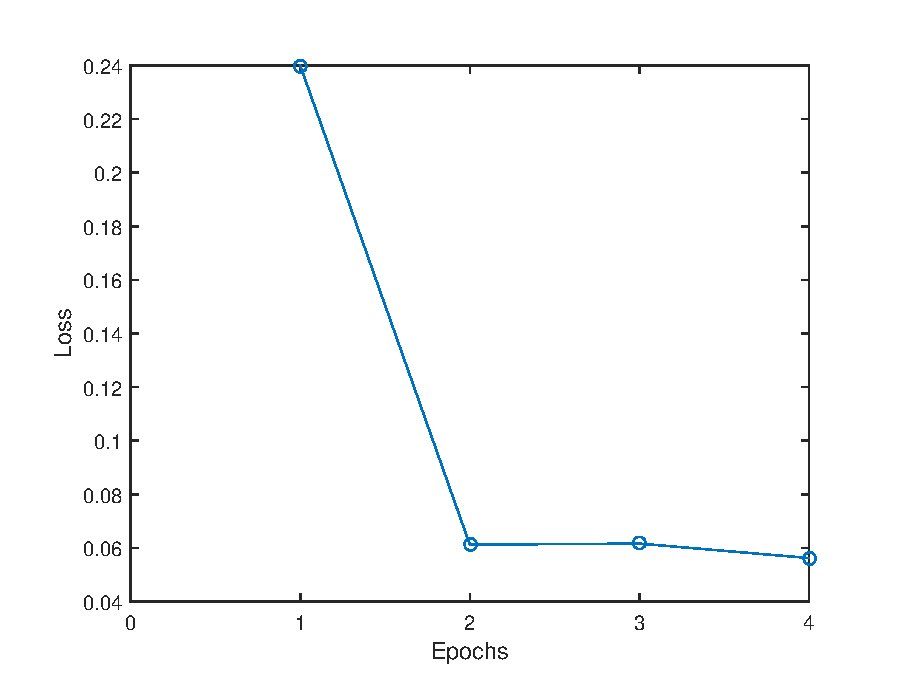
\includegraphics[height=4.7cm]{hyp_par_2}
\captionof{figure}{Change in loss function as the number of epochs is increased}
\end{minipage}

\vspace{0.2cm}

Whilst it is clear that more data means better performance, care must be taken to avoid over exposing the model to the training dataset. Failure to do so will often result in excellent performance on the training data set, but poor performance on test and validation sets due to over fitting.

\subsection{Steps Per Epoch}
The number of steps per epoch defines the number of batches of training images that go through the network in one epoch. It is considered desirable for one epoch to cover the entire dataset, and therefore this hyper-parameter can be thought of as a function of the total number of images, $N$, and the batch size, $N_{\texttt{batch}}$:
\begin{align}
	\texttt{steps\_per\_epoch} = \frac{N}{N_{batch}}
\end{align}

Setting the steps per epoch equal to the value shown in equation (2) will ensure that all of the images are covered in each epoch.

\subsection{Learning Rate}
\begin{minipage}{0.45\textwidth}
The learning rate is perhaps the most important hyper-parameter which impacts on model performance. It dictates the step size of the optimiser at each iteration. If the learning rate is `too small', then the model may fail to optimise fast enough. If the learning rate is `too big' then the model may not be able to reach optimal performance, or may fail to converge at all. The main problem in finding an acceptable learning rate is that there is no clear definition of `too big' or `too small' - the optimal learning rate is dependent on the deep learning problem.
\end{minipage}
\hspace{1cm}
\begin{minipage}{0.45\textwidth}
\centering
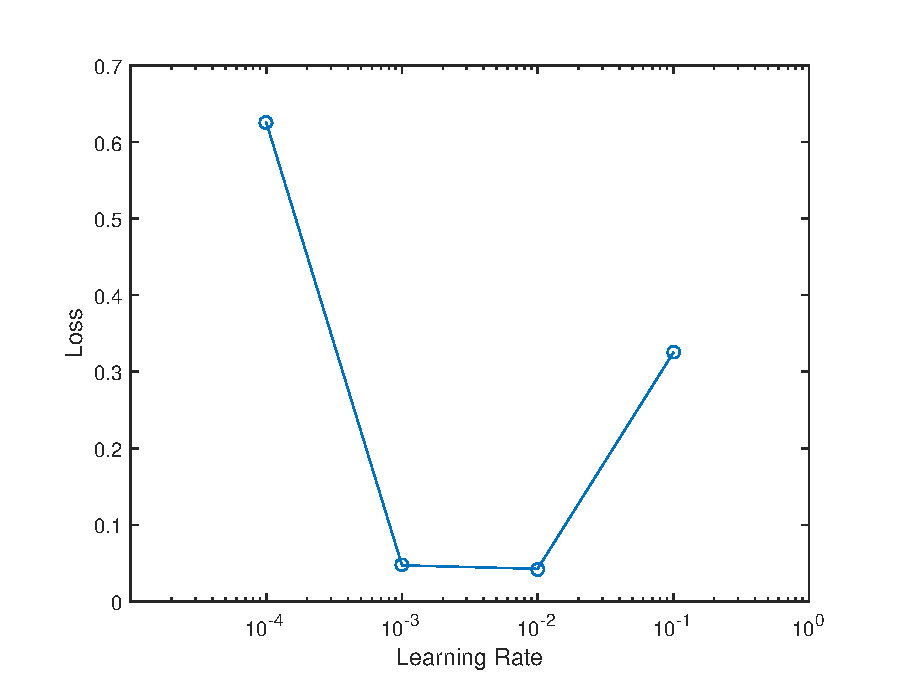
\includegraphics[height=4.7cm]{hyp_par_3}
\captionof{figure}{Change in the loss function versus change in the learning rate}
\end{minipage}

\vspace{0.2cm}

To develop some intuition on acceptable learning rates for this problem, a small experiment was conducted, looking at model performance for different learning rates, holding other hyper-parameters constant. The results can be seen in Figure 26 (note that the $x$-axis is in log scale). The experiment shows that an acceptable learning rate for this problem lies around 0.001.

\section{Results}
Models were each trained using a learning rate of 0.001, 50 epochs, with a batch size of 64, and 185 steps per epoch. The results for each of the models are presented in Sections 4.1, 4.2, and 4.3.

\subsection{Model 1 Performance}
\begin{minipage}{0.45\textwidth}
Model 1 was a `Deep' FCN Model with a single 1 $\times$ 1 convolution bridging the gap between the encoder and the decoder, shown in Section 2.3.2. Loss values over time can be seen in Figure 27, which shows rapid learning, followed by asymptotic convergence as the number of epochs increases. The evaluated intersection over union for the model was 0.3738, which fails to meet the benchmark of 0.40. Figures 28, 29, and 30 demonstrate the effectiveness of model's predictive performance, compared to the ground truth. Each Figure has three panels: the leftmost panel is the actual input, the middle panel represents perfect segmentation, and the final panel is the model segmentation.
\end{minipage}
\hspace{1cm}
\begin{minipage}{0.45\textwidth}
\centering
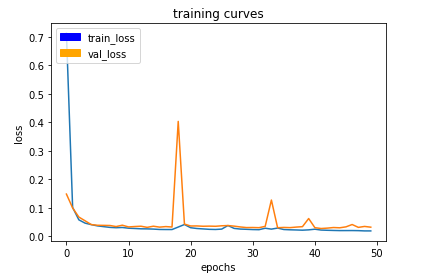
\includegraphics[scale=0.5]{Model_1}
\captionof{figure}{Loss function for each epoch during Model 1 training}
\end{minipage}

\vspace{0.5cm}

Figure 28 shows segmentation while the UAV is following the \textit{hero}; Figure 29 shows segmentation while the UAV is patrolling without the \textit{hero} in sight; and Figure 30 shows images of the UAV patrolling with the \textit{hero} in sight.
\begin{figure}[h]
\centering
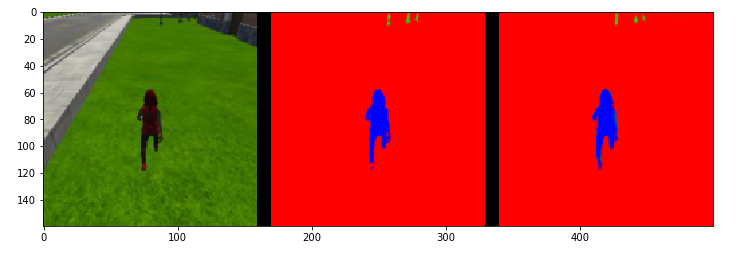
\includegraphics[scale=0.4]{model_1_1}
\caption{Model 1 segmentation while the UAV is following the \textit{hero}: the leftmost panel is the actual input, the middle panel represents perfect segmentation, and the final panel is the model segmentation}
\end{figure}

\begin{figure}[h]
\centering
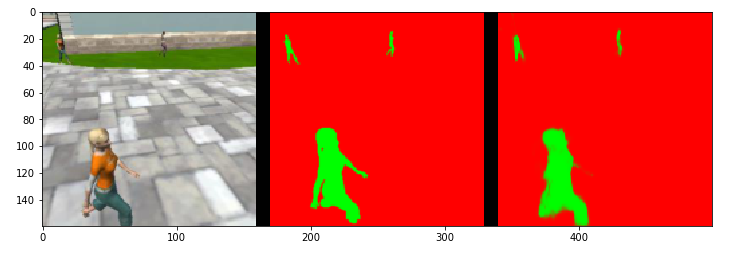
\includegraphics[scale=0.4]{model_1_2}
\caption{Model 1 segmentation while the UAV is patrolling without the \textit{hero} in sight: the leftmost panel is the actual input, the middle panel represents perfect segmentation, and the final panel is the model segmentation}
\end{figure}

\begin{figure}[h]
\centering
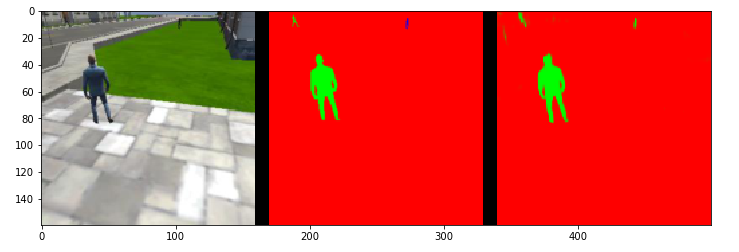
\includegraphics[scale=0.4]{model_1_3}
\caption{Model 1 segmentation while the UAV is patrolling with the \textit{hero} in sight: the leftmost panel is the actual input, the middle panel represents perfect segmentation, and the final panel is the model segmentation}
\end{figure}

\clearpage

\subsection{Model 2 Performance}
\begin{minipage}{0.45\textwidth}
Model 2 was a `Shallow' FCN Model with a single 1 $\times$ 1 convolution bridging the gap between the encoder and the decoder, shown in Section 2.3.3. Loss values over time can be seen in Figure 31, which shows rapid learning, followed by asymptotic convergence as the number of epochs increases. The evaluated intersection over union for the model was 0.3990, which fails to meet the 0.40 benchmark. Figures 32, 33, and 34 demonstrate the effectiveness of model's predictive performance, compared to the ground truth. As with Section 4.1 each figure has three panels: the leftmost panel is the actual input, the middle panel represents perfect segmentation, and the final panel is the model segmentation.
\end{minipage}
\hspace{1cm}
\begin{minipage}{0.45\textwidth}
\centering
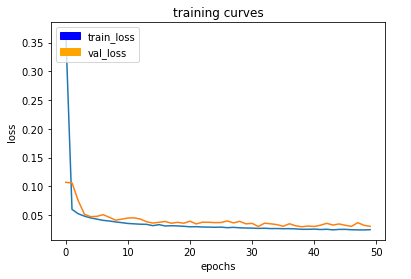
\includegraphics[scale=0.5]{Model_2}
\captionof{figure}{Loss function for each epoch during Model 1 training}
\end{minipage}

\vspace{0.5cm}

Figure 32 shows segmentation while the UAV is following the \textit{hero}; Figure 33 shows segmentation while the UAV is patrolling without the \textit{hero} in sight; and Figure 34 shows images of the UAV patrolling with the \textit{hero} in sight.
\begin{figure}[h]
\centering
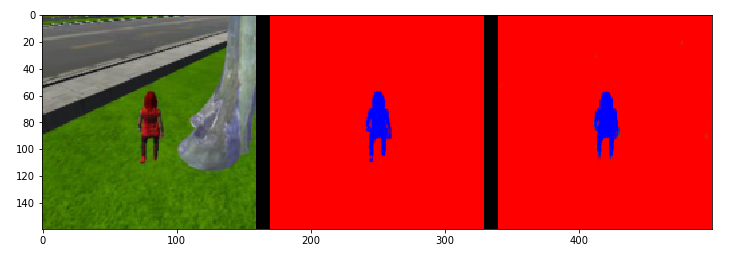
\includegraphics[scale=0.4]{model_2_1}
\caption{Model 2 segmentation while the UAV is following the \textit{hero}: the leftmost panel is the actual input, the middle panel represents perfect segmentation, and the final panel is the model segmentation}
\end{figure}

\begin{figure}[h]
\centering
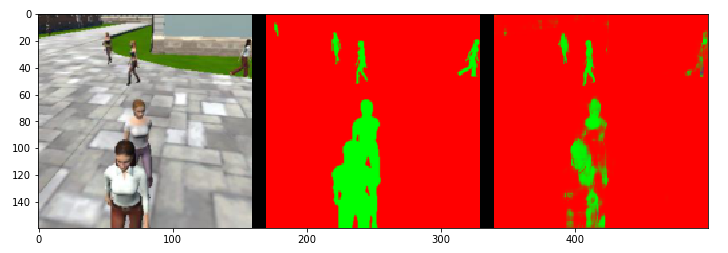
\includegraphics[scale=0.4]{model_2_2}
\caption{Model 2 segmentation while the UAV is patrolling without the \textit{hero} in sight: the leftmost panel is the actual input, the middle panel represents perfect segmentation, and the final panel is the model segmentation}
\end{figure}

\begin{figure}[h]
\centering
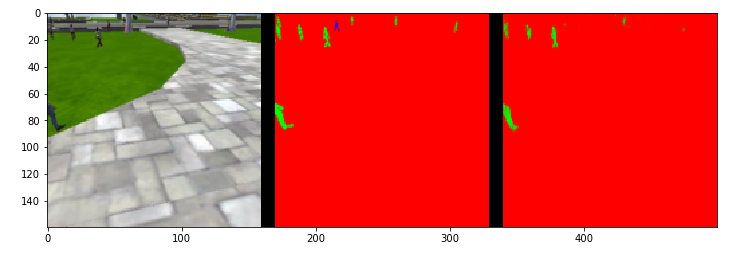
\includegraphics[scale=0.4]{model_2_3}
\caption{Model 2 segmentation while the UAV is patrolling with the \textit{hero} in sight: the leftmost panel is the actual input, the middle panel represents perfect segmentation, and the final panel is the model segmentation}
\end{figure}

\subsection{Model 3 Performance}
\begin{minipage}{0.45\textwidth}
Model 3 was a `Shallow' FCN Model without a 1 $\times$ 1 convolution bridging the gap between the encoder and the decoder, shown in Section 2.3.4. The layer between encoder and decoder a 3 $\times$ 3 convolution meaning there are more trainable parameters in the model. Loss values over time can be seen in Figure 35, which shows rapid learning, followed by asymptotic convergence as the number of epochs increases. The evaluated intersection over union for the model was 0.435, which exceeds the required 0.40 benchmark. Figures 36, 37, and 38 demonstrate the effectiveness of model's predictive performance, compared to the ground truth.
\end{minipage}
\hspace{1cm}
\begin{minipage}{0.45\textwidth}
\centering
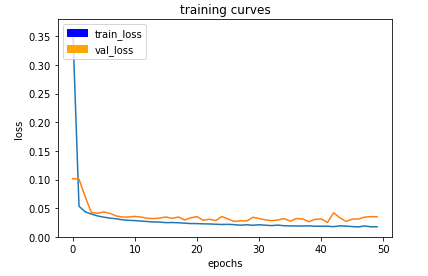
\includegraphics[scale=0.5]{Model_3}
\captionof{figure}{Loss function for each epoch during Model 1 training} 
\end{minipage}

\vspace{0.5cm}

Similarly to Section 4.1, each Figure has three panels: the leftmost panel is the actual input, the middle panel represents perfect segmentation, and the final panel is the model segmentation. Figure 36 shows segmentation while the UAV is following the \textit{hero}; Figure 37 shows segmentation while the UAV is patrolling without the \textit{hero} in sight; and Figure 38 shows images of the UAV patrolling with the \textit{hero} in sight.
\begin{figure}[h]
\centering
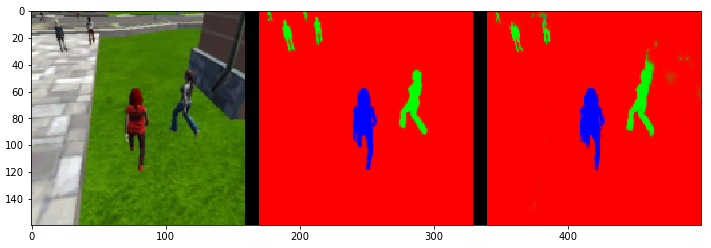
\includegraphics[scale=0.4]{model_3_1}
\caption{Model 3 segmentation while the UAV is following the \textit{hero}: the leftmost panel is the actual input, the middle panel represents perfect segmentation, and the final panel is the model segmentation}
\end{figure}

\begin{figure}[h]
\centering
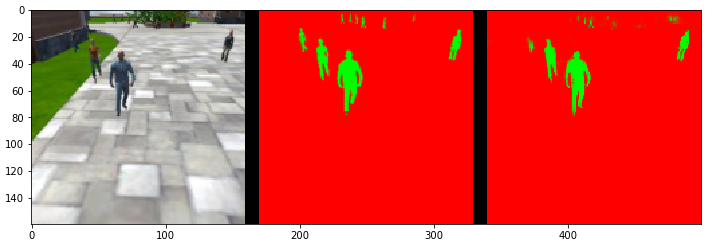
\includegraphics[scale=0.4]{model_3_2}
\caption{Model 3 segmentation while the UAV is patrolling without the \textit{hero} in sight: the leftmost panel is the actual input, the middle panel represents perfect segmentation, and the final panel is the model segmentation}
\end{figure}

\begin{figure}[h]
\centering
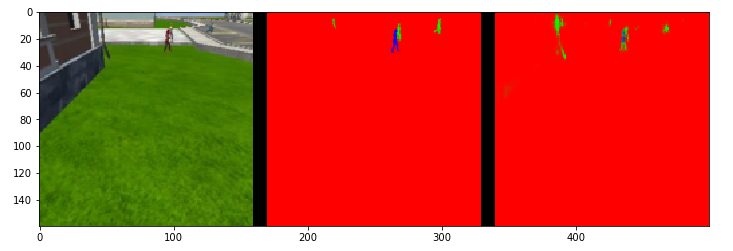
\includegraphics[scale=0.4]{model_3_3}
\caption{Model 3 segmentation while the UAV is patrolling with the \textit{hero} in sight: the leftmost panel is the actual input, the middle panel represents perfect segmentation, and the final panel is the model segmentation}
\end{figure}

\newpage

\section{Discussion \& Future Enhancements}
Three separate FCN models were trained to provide pixel by pixel segmentation of images from a 3D simulation. All three models were able to provide some level of segmentation, however, only the model which didn't use 1 $\times$ 1 convolutions was able to achieve the required intersection over union benchmark. It is unclear why this may be the case - using a 3 $\times$ 3 convolution instead of a 1 $\times$ 1 convolution adds additional parameters to the models, however, adding additional parameters by making the model deeper (as with Model 1) failed to produce similar results. To better understand how the models work for this task, and to improve model performance, there are a number of areas that could be explored. These include:
\begin{itemize}
\item Increasing the patch sizes to include larger patches (e.g. 5 $\times$ 5)
\item Adding pooling layers in the encoder, and unpooling layers in the decoder
\item Increasing the depth of the model and getting a larger dataset - additional images could be achieved by flipping all of the current images
\item Increasing the number of epochs for which the model is trained
\item Adding regularisation to the model with dropout
\end{itemize}

\newpage

\section{References}




Badrinarayanan, V., Kendall, A., \& Cipolla, R. (2016). SegNet: A Deep Convolutional Encoder-Decoder Architecture for Image Segmentation. \textit{arXiv:1511.00561v3}\\

Ciresan, D. C., Meier, U., Gambardella, L. M., \& Schmidhuber, J. (2010). Deep Big Simple Neural Nets Excel on Handwritten Digit Recognition. \textit{arXiv:1003.0358v1}.\\

He, K., Zhang, X., Ren, S., \& Sun, J. (2015). Deep Residual Learning or Image Recognition. \textit{arXiv:1512.03385v1}\\

Huang, T. S. (1996). Computer Vision: Evolution and Promise, University of Illinois at Urbana-Champaign\\

Ioffe, S., \& Szegedy, C. (2015). Batch Normalization: Accelerating Deep Network Training by Reducing Internal Covariate Shift. \textit{arXiv:1502.031167v3}\\

Krizhevsky, A., Sutskever, I., \& Hinton, G. E. (2012). ImageNet Classification with Deep Convolutional Neural Networks. \textit{Advances in Neural Information Processing Systems 25 (NIPS 2012)}\\

Lin, M., Chen, Q., \& Yan, S. (2014). Network in Network. \textit{arXiv:1312.4400v3}\\

Long, J., Shelhamer, E., \& Darrell, T. (2014). Fully Convolutions Networks for Semantic Segmentation, 	\textit{arXiv:1411.4038}.\\

Ruder, S. (2017). An overview of gradient descent optimization algorithms. \textit{arXiv:1609:04747v2}\\

Yann, L., Botton, L., Bengio, Y., \& Haffner, P. (1998). Gradient-Based Learning Applied to Document Recognition,\textit{Proceedings of the IEEE}, DOI: 10.1109/5.726791.\\

\end{document}